%----------------------------------------------------------------------------
\chapter{Áttekintés}\label{chapter:overview}
%----------------------------------------------------------------------------
%Mit csinál
%Mire jó (szerkesztés, finomítás?, import? új objektumok...)
%(technológia nélkül)

\section{Parciális modell szerkesztő funkciói}
Parciális modell szerkesztő funkciói
Kutatásom során megnéztem egy másik modellezőeszközt, ami a 'May' részlegesség feloldására nyújt megoldást és ezzel kapcsolatos döntéstámogatást szolgáltat\cite{Michalis}. A többi részlegesség kezelését nem teszi lehetővé. célom egy olyan modellező eszköz elkészítése, ami segítségével lehetséges részleges modelleket készíteni. Ehhez olyan vizuális szerkesztőfelület társul, ami megkönnyíti ezt a folyamatot. Ahhoz, hogy ez generikusan működjön egy általános modell szükséges. Így ez a modell tartalmazni fog objektumokat, attribútumokat és az ezek közti kapcsolatot kifejező referenciákat. Ezen felül minden elemhez lehetséges rendelni \textit{May}, \textit{Var} vagy \textit{Abs} részlegességet. Magához a modellhez pedig \textit{OW} részlegességet lehet rendelni.
\par
A kapcsolódó editor képes részleges modellt létrehozni és manipulálni. Lehetőséget ad új objektumok, attribútumok, referenciák létrehozására. Ezen elemekhez a már fent említett részlegességek rendelhetők. Objektumhoz hozzárendelve a 'May' vagy 'Abs' részlegességet az a benne lévő attribútumokra, illetve a hozzá tartozó összes referenciára érvényes lesz. 'Var' annotáció esetén ez csak az objektumra vonatkozik. Attribútumnál mindhárom részlegesség csak önmagára értelmezzük. Referencia esetén szintén csak saját magára értelmezett a részlegesség. A szerkesztő a részlegességek feloldására, tehát finomításra is biztosít eszközöket, figyelembe véve az előbbi értelmezéseket. Például egy 'May' részlegesség feloldása egy objektumnál nem csak magát az objektumot törli, hanem referenciáit és attribútumait is.(áttekintő ábra lásd \autoref{overview})



\begin{figure}[!ht]
	\centering
	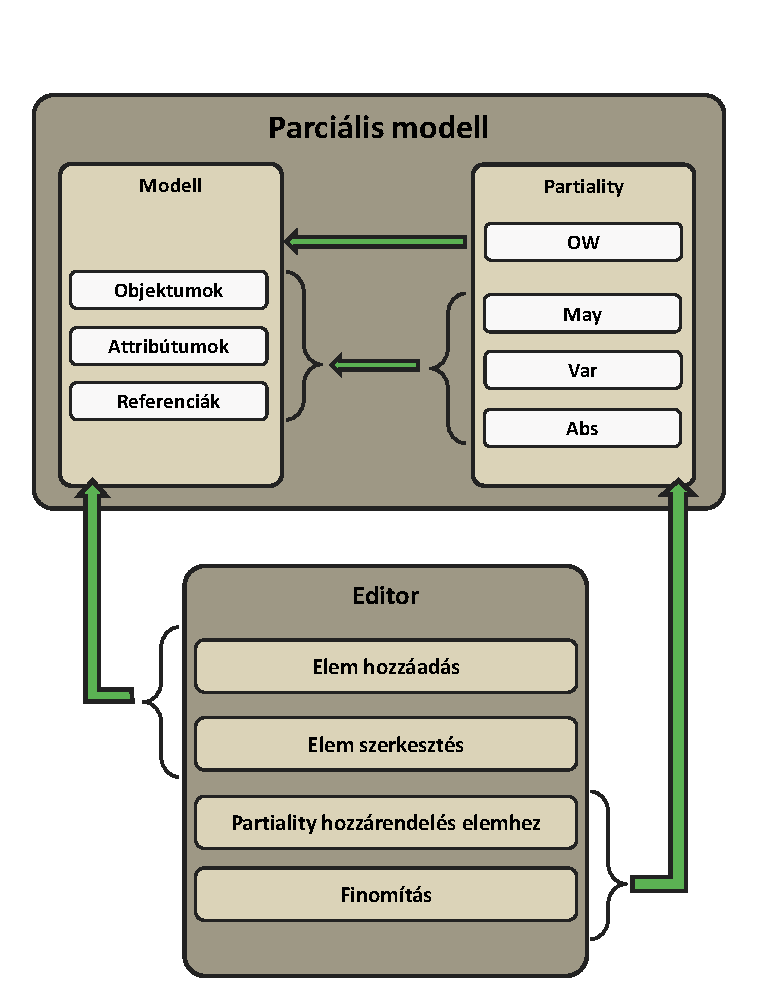
\includegraphics[width=100mm]{figures/overview.pdf}
	\caption{Részleges modell és a rajta végezhető műveletek} 
	\label{overview}
\end{figure}


\section{Fejlesztési lehetőségek}
Egy általános osztálydiagram 'tree editor'-ban való szerkesztése sok dologra nem nyújt lehetőséget. 
Nem létezhet például attribútum objektum nélkül. Attribútumot nem lehet több objektumhoz is hozzákapcsolni. Tehát kizárólag érvényes modelleket lehet készíteni benne. Azonban a modell tervezése folyamán nem feltétlenül szükséges, hogy ilyen megkötések legyenek. A részleges modell szerkesztésénél nincsenek ilyen feltételek. Lehetséges attribútumot létrehozni objektum nélkül, vagy több objektumhoz is hozzá lehet kapcsolni anélkül, hogy ez konfliktust okozna a szerkesztőnek.
\par
Részleges modell lehetőséget biztosíthat arra is, hogy példányosítsunk absztrakt osztályokat. Ugyanis egy absztrakt osztály becsomagolható a parciális modell egy objektumába, ezáltal viselkedése megváltozhat. 
\par
Egy objektumdiagram esetében a multiplicitás korlátos. Tehát van vagy minimum vagy maximum megszorítás, akkor ezek nem hághatóak át. Tegyük fel, hogy egy 'A' objektum legfeljebb egy 'B' típusú objektumot tartalmazhat. 'B1' és 'B2' is 'B' típusú. Kezdetben nem tudjuk eldönteni még, hogy melyik objektum lesz a modellben akkor nincs lehetőségünk mindkettőt létrehozni, hogy majd később dönthessük el a sorsukat, hanem az egyiket mindenképp el kell hagyni. Részleges modell ennél megengedőbb és ha szükséges 'B1' és 'B2' objektum is kapcsolódhat 'A' objektumhoz.

\section{Esettanulmány}
A következő példában bemutatom, hogy egy parciális modellszerkesztő milyen lehetőségeket biztosít. Tételezzük fel, hogy egy már meglévő modellt 'M' szeretnénk parciális modellként kezelni. Ehhez az első lépés, hogy importáljuk a modellt. Ez azt jelenti, hogy minden egyes elemét (Objektum, attribútum, referencia) megfeleltetjük egy részleges modellbeli elemmel (lásd \autoref{import}). A következő ábra jól szemlélteti ezt. Az így kapott eredmény egy parciális modell, amit nevezzünk 'PM'-nek.
\begin{figure}[!ht]
	\centering
	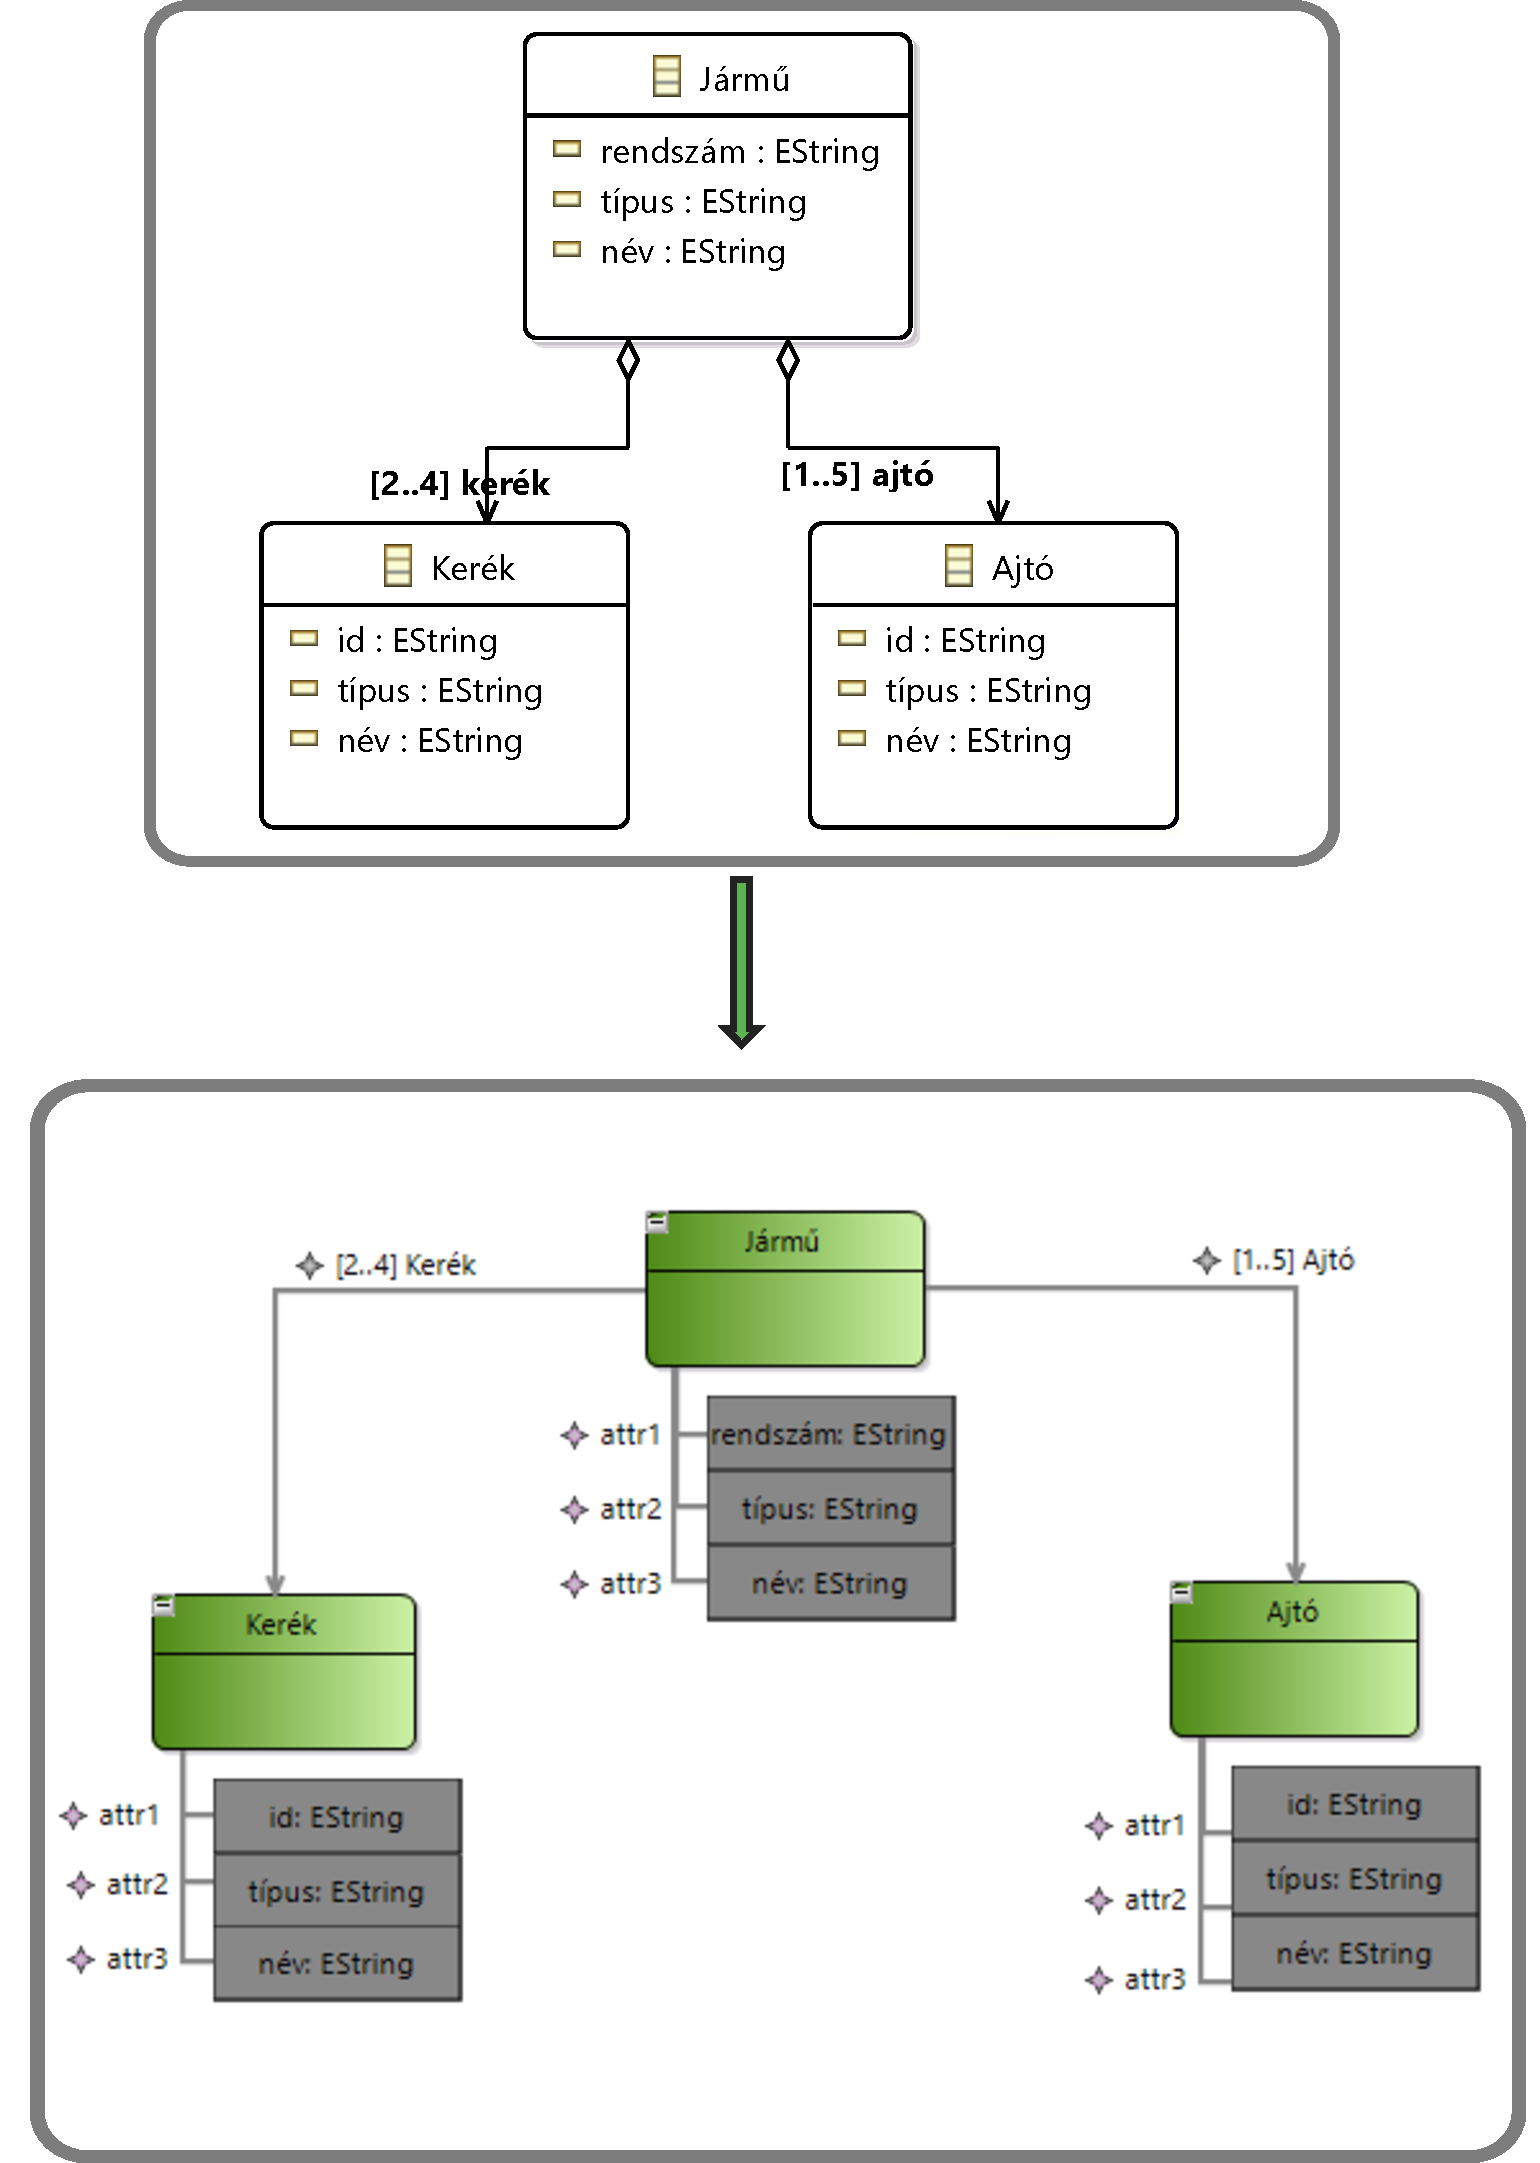
\includegraphics[width=100mm]{figures/pl01.pdf}
	\caption{Osztálydiagram megfeleltetése parciális modellel} 
	\label{import}
\end{figure}
\par
Következő lépésben módosíthatjuk a modellt. Például adhatunk hozzá új elemet(TODOÁBRA). A részleges modellbeli objektumban el van tárolva, hogy az milyen típusú így nem különbözik a már meglévő elemektől. Ez fontos lesz majd, ha vissza szeretnénk konvertálni nem parciális modell elemmé. Elemet törölni is lehet. Egyik objektum attribútumát eltávolíthatjuk például(TODOÁBRA).
\par
Eddigi módosításokhoz még nem kellett a részleges modell lehetőségeit felhasználni, ezt az eredeti modellben is megtehettük volna. Most viszont egy attribútumot hozzáadunk a modellhez anélkül, hogy az bármelyik objektumhoz is kapcsolódna. (TODOÁBRA) Ezután ezt az attribútumot mivel még nem tudjuk  hova is tartozzon dönthetünk úgy hogy több objektumhoz is hozzákapcsoljuk. (TODOÁBRA)
Jelen pillanatban akkor van egy attribútumunk, ami két különböző objektumban is benne van. Ez azonban a végleges modellben biztosan nem maradhat így, mert nem lehetne visszaexportálni 'M' modellé, ugyanis az nem kezel ilyen esetet. Hogy ezt ne keljen fejben tartanunk meg tudjuk jelölni. Tehetünk az attribútumra egy 'May' annotációt mind a két objektum részéről. A szemléltető ábrán ez úgy van ábrázolva, hogy az attribútumot és objektumot összekötő vonalat megjelöljük (MayExist) (TODOÁBRA). Így a modellre rátekintve leolvasható, hogy van egy attribútum aminek nem tudjuk a pontos hovatartozását.(???var vagy abs esetleg)
\par
A modellt lehetséges finomítani és szükséges is, ha vissza szeretnénk nyerni egy 'M'-el megegyező típusú modellt. Finomítás következtében eltüntethetjük az annotációkat és azokkal együtt a bizonytalanságokat is. Első lépésben finomítsuk az attribútumot. Fixáljuk le, hogy melyik objektumhoz fog tartozni.(TODOÁBRA)
\par
Végül, ha már a modellünk nem tartalmaz részlegességet akkor vissza is alakíthatjuk az eredeti 'M' modell típusával megegyező típusú modellé.(TODOÁBRA)